\subsection{Opdracht 02b}

\paragraph{
Een mooier alternatief is een statement dat per land de percentages en totalen geeft over een jaar in kolommen.
}

\begin{lstlisting}
    -- jouw statement hier levert b.v. onderstaand resultaat voor 2017

    Countryname  January	Feburary  March    April    May    June    July    August  September  October  November  December  TotalItems
    Chile         9.76%    8.22%   10.06%    9.07%   9.26%   8.38%   8.91%    7.75%    7.28%     7.09%     7.53%    6.68%     3638
    Greece        9.67%    7.69%    9.06%    8.49%   8.49%   7.92%   9.06%    8.49%    8.40%     7.78%     7.78%    7.17%     2120
    Poland        9.93%    7.94%    9.41%    8.82%   8.82%   8.24%   8.24%    7.72%    7.72%     7.72%     7.72%    7.72%     1360
    Netherlands   8.38%    7.26%    8.94%    8.38%   8.38%   7.82%   8.94%    8.38%    8.38%     8.38%     8.38%    8.38%      716
\end{lstlisting}

\subsubsection{Versie 01}
TODO: Nick
\lstinputlisting[language=SQL]{sql/nick/opdracht-01-02b-v1.sql}
\begin{figure}[H]
    \centering
    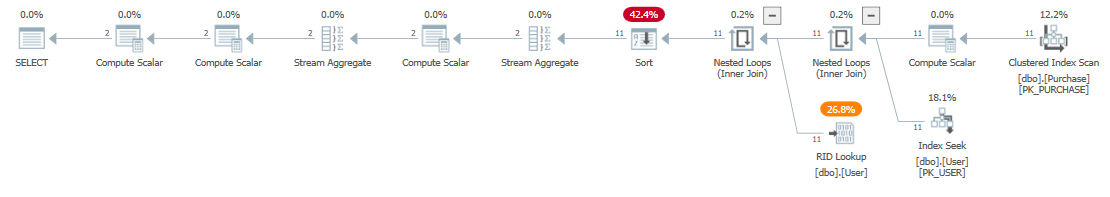
\includegraphics[width=1\textwidth]{image/nick/opdracht-02b.PNG}
    \caption{Queryplan Opdracht 02b Versie 01}
\end{figure}

\subsubsection{Versie 02}
TODO: Marc
\lstinputlisting[language=SQL]{sql/marc/opdracht-01-02b.sql}
\begin{figure}[H]
    \centering
    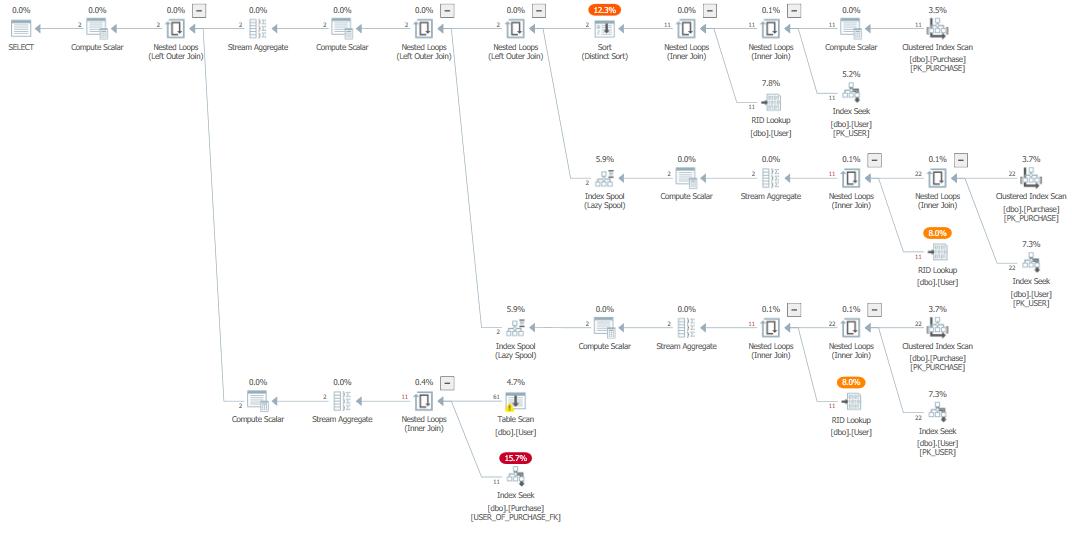
\includegraphics[width=1\textwidth]{image/marc/opdracht-02b.PNG}
    \caption{Queryplan Opdracht 02b Versie 02}
\end{figure}

\subsection{Conclusie}
Versie 01 presteert met 22\% van de totale duur van de gehele batch aanzienlijk sneller dan versie 02 welke 78\% van de duur nodig heeft.
Uit het queryplan wordt duidelijk dat versie 02 in het beginstadium iets beter presteert. Deze voert een 'Index Seek (NonClustered)' uit
voor 2 van de 11 records in de User tabel. Hetzelfde geldt voor de 'RID Lookup (Heap)' welke eveneens voor 2 van de 11 records informatie
uit de User tabel ophaalt. Na deze stap doorloopt versie 01 echter een eenvoudig proces zonder extra 'Nested Loops' en de extra ballast
welke hieraan vooraf gaat zoals een 'Filter', 'Clustered Index Scan' en een 'Table Scan'. Derhalve kan worden gesteld dat versie 01
beter preseteert dan versie 02. De onderhoudbaarheid van versie 01 is eveneens beter dan die van versie 02, niet alleen omdat de structuur
helder en overzichtelijk is, maar ook vanwege het gebruik van een CTE waardoor een duidelijke resultset terug wordt gegeven.